% !TEX encoding = UTF-8
% !TEX TS-program = pdflatex
% !TEX root = ../tesi.tex

%**************************************************************
\chapter{Introduzione}
\label{cap:introduzione}
%**************************************************************

Introduzione al contesto applicativo.\\

\noindent Esempio di utilizzo di un termine nel glossario \\
\gls{api}. \\

\noindent Esempio di citazione in linea \\
\cite{site:agile-manifesto}. \\

\noindent Esempio di citazione nel pie' di pagina \\
citazione\footcite{womak:lean-thinking} \\

%**************************************************************
\section{SyncLab }
SyncLab è una Innovative Company collocata in tutta italia, è nata nel 2002 con sede principale a Napoli ed è cresciuta velocemente. Attualmente, SyncLab ha 6 sedi in tutta italia, più di 300 dipendenti e più di 150 clienti diretti e finali.\\
SyncLab propone servizi Innovativi che aiutano i clienti nella realizzazione, progettazione e manutenzioni di soluzioni IT, sia dal punto di vista tecnologico, sia nel Governo del Cambiamento Organizzativo.
L'azienda ha collobarobato con vari compagnie tra questi i più importanti sono: Tim, Trenitalia, HM, Grimaldi Lines, notartel, sky, eni, enel, vodafone, RayWay, Poste Italiane, Intesa Sanpaolo, Ministero dell'economia delle finanze, fastweb e UniCredit.
\begin{figure}[H]
    \centering
    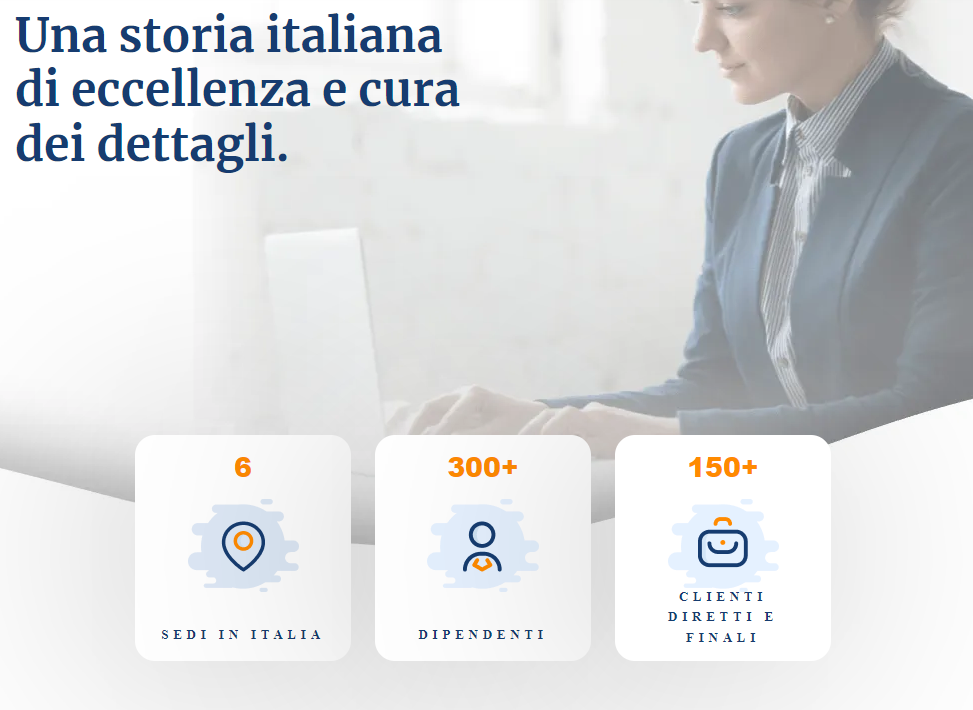
\includegraphics[scale=0.50]{azienda.png}
    \caption{Punti di forza di SyncLab}
\end{figure}
\subsection{Prodotti}
Come accenato, SyncLab opera nel settore IT e i suoi prodotti nascono dalle competenze acquisite e maturate durante le loro 20 anni di collaborazioni. I prodotti coprono vari ambiti come quelli delle telecomunicazioni, utilities, finanza e salute.
\begin{figure}[H]
    \centering
    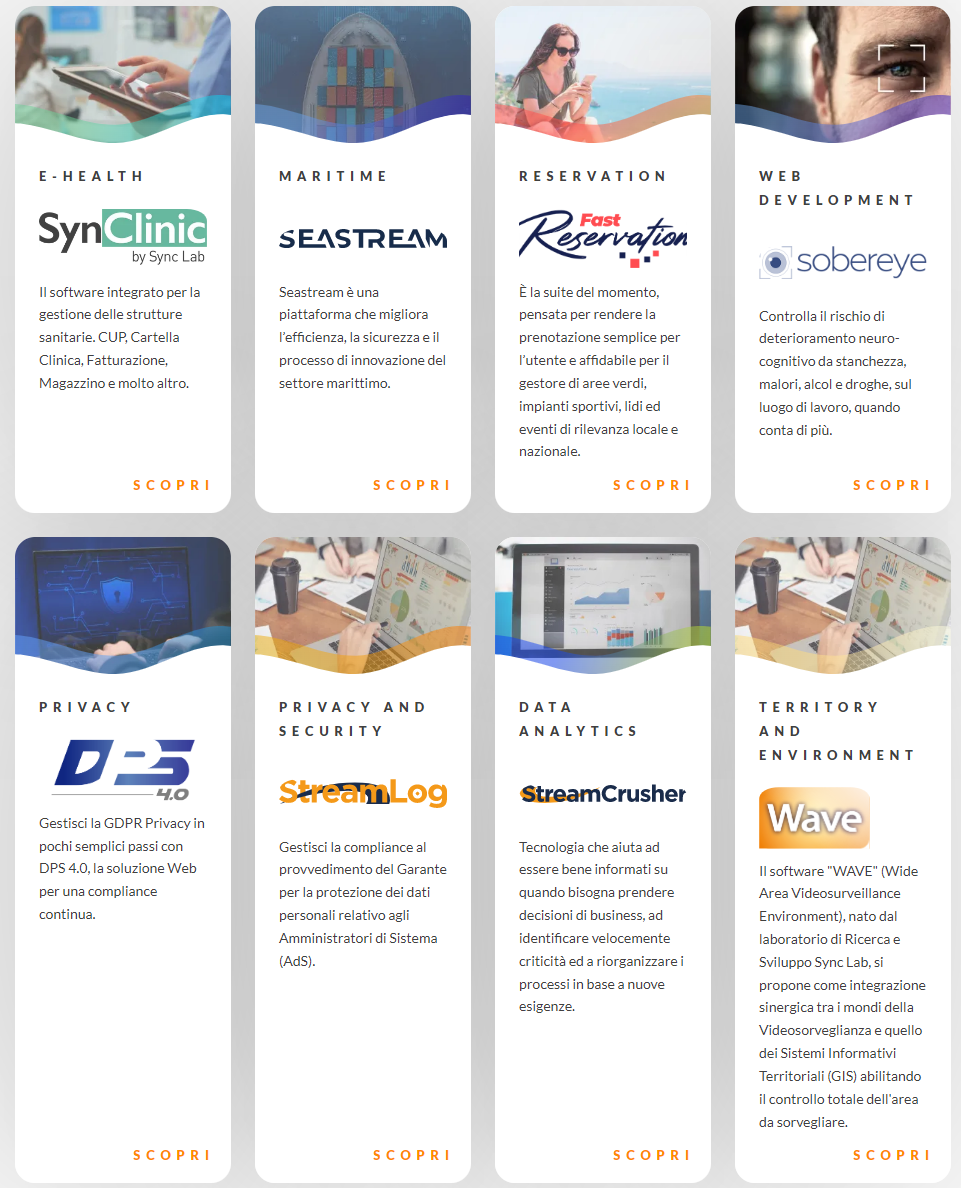
\includegraphics[width=1.0\textwidth]{prodotti.png}
    \caption{I vari prodotti di SyncLab}
\end{figure}
\begin{itemize}
    \item \textbf{SynClinic:} software integrato per la gestione delle strutture sanitarie, come il sistema di cartella clinica digitale, il servizio di fatturazione, la gestione informatizzata dei farmaci, i strumenti nativi di gestione amministrativa e tanto altro.
    \item \textbf{SEASTREAM:} una piattaforma nata per migliorare e potenziare le attività di business nel settore armatoriali e di altri operatori del mercato marittimo
    \item \textbf{FastReservation:} applicazione realizzato per rendere il sistema di prenotazione più facile e affidabile per gli utenti.
    \item \textbf{sobereye:} soluzione per la sicurezza proattiva per la prevenzione degli incidenti nei settori di trasporti, estrazione, costruzioni e industrale.
    \item \textbf{DPS 4.0:} applicativo che permette di gestire la GDPR Privacy Policy. L'applicativo, tramite una guida semplice sviluppata dagli ingegneri esperti nell'ambito dei user experience, offre la possibilità di modificare e aggiornare i documenti sulla privacy con il minimo sforzo.
    \item \textbf{StreamLog:} soluzione per la protezione dei dati personali relativo agli Amministratori di Sistema, dà possibilità di effettuare il controllo degli accessi degli utenti ai sistemi in modo semplice ed efficace.
    \item \textbf{StreamCrusher:} tecnologia che serve per aiutare a prendere decisioni di business, indentificando velocemente i punti critici e riformando i processi in base alle nuove esigenze.
    \item \textbf{Wave:} software nato per i sistemi di vidersorverglianza, con l'obiettivo di avere una maggiore copertura territoriale col minor numero di telecamere installate e possibilmente utilizzare il minor numero possibile di risorse.
\end{itemize}
%**************************************************************


%**************************************************************
\section{Organizzazione del testo}

\begin{description}
    \item[{\hyperref[cap:il progetto di stage]{Il secondo capitolo}}] descrive ...
    
    \item[{\hyperref[cap:analisi dei requisiti]{Il terzo capitolo}}] approfondisce ...
    
    \item[{\hyperref[cap:progettazione e codifica]{Il quarto capitolo}}] approfondisce ...
    
    \item[{\hyperref[cap:progettazione-codifica]{Il quinto capitolo}}] approfondisce ...
    
    \item[{\hyperref[cap:verifica-validazione]{Il sesto capitolo}}] approfondisce ...
    
    \item[{\hyperref[cap:conclusioni]{Nel settimo capitolo}}] descrive ...
\end{description}

Riguardo la stesura del testo, relativamente al documento sono state adottate le seguenti convenzioni tipografiche:
\begin{itemize}
	\item gli acronimi, le abbreviazioni e i termini ambigui o di uso non comune menzionati vengono definiti nel glossario, situato alla fine del presente documento;
	\item per la prima occorrenza dei termini riportati nel glossario viene utilizzata la seguente nomenclatura: \emph{parola}\glsfirstoccur;
	\item i termini in lingua straniera o facenti parti del gergo tecnico sono evidenziati con il carattere \emph{corsivo}.
\end{itemize}